\iffalse
This file is protected by Copyright. Please refer to the COPYRIGHT file
distributed with this source distribution.

This file is part of OpenCPI <http://www.opencpi.org>

OpenCPI is free software: you can redistribute it and/or modify it under the
terms of the GNU Lesser General Public License as published by the Free Software
Foundation, either version 3 of the License, or (at your option) any later
version.

OpenCPI is distributed in the hope that it will be useful, but WITHOUT ANY
WARRANTY; without even the implied warranty of MERCHANTABILITY or FITNESS FOR A
PARTICULAR PURPOSE. See the GNU Lesser General Public License for more details.

You should have received a copy of the GNU Lesser General Public License along
with this program. If not, see <http://www.gnu.org/licenses/>.
\fi

\documentclass{article}
\author{} % Force author to be blank
%----------------------------------------------------------------------------------------
% Paper size, orientation and margins
%----------------------------------------------------------------------------------------
\usepackage{geometry}
\geometry{
  letterpaper,      % paper type
  portrait,       % text direction
  left=.75in,       % left margin
  top=.75in,        % top margin
  right=.75in,      % right margin
  bottom=.75in      % bottom margin
 }
%----------------------------------------------------------------------------------------
% Header/Footer
%----------------------------------------------------------------------------------------
\usepackage{fancyhdr} \pagestyle{fancy} % required for fancy headers
\renewcommand{\headrulewidth}{0.5pt}
\renewcommand{\footrulewidth}{0.5pt}
\rhead{\small{ANGRYVIPER Team}}
%----------------------------------------------------------------------------------------
% Appendix packages
%----------------------------------------------------------------------------------------
\usepackage[toc,page]{appendix}
%----------------------------------------------------------------------------------------
% Defined Commands & Renamed Commands
%----------------------------------------------------------------------------------------
\renewcommand{\contentsname}{Table of Contents}
\renewcommand{\listfigurename}{List of Figures}
\renewcommand{\listtablename}{List of Tables}
\newcommand{\todo}[1]{\textcolor{red}{TODO: #1}\PackageWarning{TODO:}{#1}} % To do notes
\newcommand{\code}[1]{\texttt{#1}} % For inline code snippet or command line
%----------------------------------------------------------------------------------------
% Various pacakges
%----------------------------------------------------------------------------------------
\usepackage{hyperref} % for linking urls and lists
\usepackage{graphicx} % for including pictures by file
\usepackage{listings} % for coding language styles
\usepackage{rotating} % for sideways table
\usepackage{pifont}   % for sideways table
\usepackage{pdflscape} % for landscape view
%----------------------------------------------------------------------------------------
% Table packages
%----------------------------------------------------------------------------------------
\usepackage{longtable} % for long possibly multi-page tables
\usepackage{tabularx} % c=center,l=left,r=right,X=fill
\usepackage{float}
\floatstyle{plaintop}
\usepackage[tableposition=top]{caption}
\newcolumntype{P}[1]{>{\centering\arraybackslash}p{#1}}
\newcolumntype{M}[1]{>{\centering\arraybackslash}m{#1}}
%----------------------------------------------------------------------------------------
% Block Diagram / FSM Drawings
%----------------------------------------------------------------------------------------
\usepackage{tikz}
\usetikzlibrary{shapes,arrows,fit,positioning}
\usetikzlibrary{automata} % used for the fsm
%----------------------------------------------------------------------------------------
% Colors Used
%----------------------------------------------------------------------------------------
\usepackage{colortbl}
\definecolor{blue}{rgb}{.7,.8,.9}
\definecolor{ceruleanblue}{rgb}{0.16, 0.32, 0.75}
\definecolor{drkgreen}{rgb}{0,0.6,0}
\definecolor{deepmagenta}{rgb}{0.8, 0.0, 0.8}
\definecolor{cyan}{rgb}{0.0,0.6,0.6}
\definecolor{maroon}{rgb}{0.5,0,0}
%----------------------------------------------------------------------------------------
% Update the docTitle and docVersion per document
%----------------------------------------------------------------------------------------
\def\docTitle{Component Data Sheet}
\def\docVersion{1.4}
%----------------------------------------------------------------------------------------
\date{Version \docVersion} % Force date to be blank and override date with version
\title{\docTitle}
\lhead{\small{\docTitle}}

\def\comp{fifo}
\edef\ecomp{fifo}
\def\Comp{FIFO}
\graphicspath{ {figures/} }

\begin{document}

\section*{Summary - \Comp}
\begin{tabular}{|c|M{13.5cm}|}
  \hline
  \rowcolor{blue}
                    &                                                              \\
  \hline
  Name              & \comp                                                        \\
  \hline
  Worker Type       & Application                                                  \\
  \hline
  Version           & \docVersion                                                 \\
  \hline
  Release Date      & October 2018                                              \\
  \hline
  Component Library & ocpi.assets.util\_comps                                        \\
  \hline
  Workers           & \comp.hdl                                                    \\
  \hline
  Tested Platforms  & isim \\
  \hline
\end{tabular}

\section*{Functionality}
\begin{flushleft}
  The FIFO component passes complex signed samples (Q0.15 I, Q0.15 Q) from the input port through a First-In-First-Out (FIFO) buffer and onward to the output port. The depth, in number of complex samples, of the FIFO buffer is parameterized. This component includes a property-driven oneshot mode which, when enabled, allows the first FIFO depth number of samples to be sent to the output port and then disontinues data flow to the output port. After data flow is discontinued, the input port still ingests available samples, effectively operating as a data sink. This worker can also be parameterized to send a Zero-Length Message (ZLM) once data flow is discontinued.
\end{flushleft}

\section*{Worker Implementation Details}
\subsection*{\comp.hdl}
\begin{flushleft}
  In keeping with good data flow control practices, backpressure is transferred, when necessary, from the output port to the input port. Backpressure is never transferred when in oneshot mode and after the data flow is discontinued. Backpressure from the output port and forwardpressure from the input port are both alleviated by the FIFO buffer, with the degree of alleviation being directly proportional to the parameterized depth of the FIFO buffer (\verb+FIFO_DEPTH_p+).\medskip

  The input port's SOM, EOM, byte\_enable, and valid indicators are passed through the FIFO to the output port when data flow is allowed. Consequently, ZLMs will be passed through this worker. If operating in oneshot mode and data flow has been discontinued, the EOM will be set (i.e. logic value of 1 applied) on the same clock pulse as the last output sample.\medskip

  The \verb+ZLM_WHEN_ONESHOT_DONE_p+ parameter property, when having a value of true, forces the worker to send a single ZLM when in oneshot mode and data flow has been discontinued (i.e. when oneshot is 'done'). This is useful for allowing applications which use this worker to terminate once data flow is discontinued.
\end{flushleft}

\section*{Block Diagrams}
\subsection*{Top level}
\begin{center}
  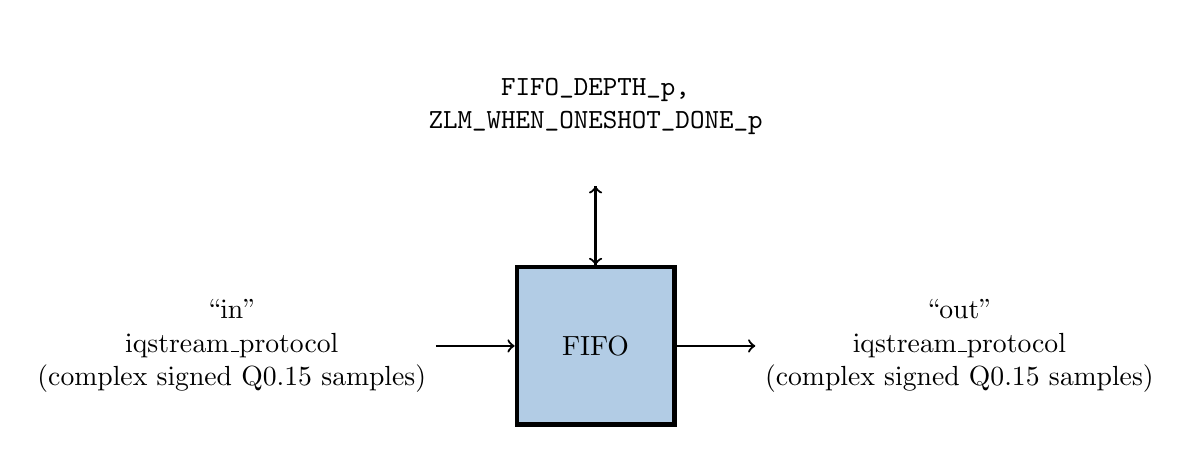
\begin{tikzpicture}[% List of styles applied to all, to override specify on a case-by-case
      every node/.style={
        align=center,     % use this so that the "\\" for line break works
        minimum size=2cm  % creates space above and below text in rectangle
      },
      every edge/.style={draw,thick}
    ]
    \node[rectangle,ultra thick,draw=black,fill=blue](R2){\Comp};
    \node[rectangle,draw=white,fill=white](R3)[left= of R2]{``in'' \\ iqstream\_protocol \\ (complex signed Q0.15 samples) };
    \node[rectangle,draw=white,fill=white](R4)[right= of R2]{``out'' \\ iqstream\_protocol \\ (complex signed Q0.15 samples) };
    \node[rectangle,draw=white,fill=white](R5)[above= of R2]{\verb+FIFO_DEPTH_p,+ \\ \verb+ZLM_WHEN_ONESHOT_DONE_p+};
    \path[->]
    (R3)edge [] node [] {} (R2)
    (R2)edge [] node [] {} (R4)
    (R2)edge [] node [] {} (R5)
    (R5)edge [] node [] {} (R2)
    ;
  \end{tikzpicture}
\end{center}

\section*{Source Dependencies}
\subsection*{\comp.hdl}
\begin{itemize}
  \item assets/components/util\_comps/fifo.hdl/fifo.vhd
  \item core/hdl/primitives/bsv/bsv\_pkg.vhd
  \item core/hdl/primitives/bsv/imports/SizedFIFO.v
\end{itemize}

\begin{landscape}
  \section*{Component Spec Properties}
  \begin{scriptsize}
    \begin{tabular}{|p{4cm}|p{1cm}|p{2cm}|p{2cm}|p{2cm}|p{2cm}|p{1cm}|p{5.5cm}|}
      \hline
      \rowcolor{blue}
      Name               & Type   & SequenceLength & ArrayDimensions   & Accessibility       & Valid Range                                                                      & Default & Usage                                                                        \\
      \hline
      \verb+FIFO_DEPTH_p+  & ULong  & -              & -                 & Parameter & Standard                                                                              & 1024      & Maximum number of complex samples which the FIFO can hold at any given time. \\
      \hline
      \verb+ZLM_WHEN_ONESHOT_DONE_p+        & Bool  & -              & -                 & Readable, Initial            & Standard                                                                         & False       & When true, worker will generate Zero-Length-Message after oneshot was enabled and completed. \\
      \hline
    \end{tabular}
  \end{scriptsize}

  \section*{Worker Properties}
  \subsection*{\comp.hdl}
  \begin{scriptsize}
    \begin{tabular}{|p{3cm}|p{2cm}|p{1cm}|p{2cm}|p{2cm}|p{2cm}|p{2cm}|p{3cm}|p{2cm}|}
      \hline
      \rowcolor{blue}
      Type     & Name                 & Type  & SequenceLength & ArrayDimensions & Accessibility       & Valid Range & Default & Usage                                        \\
      \hline
      - & -  & - & -              & -               & - & -        & -      & -\\
      \hline
    \end{tabular}
  \end{scriptsize}


  \section*{Component Ports}
  \begin{scriptsize}
    \begin{tabular}{|p{2cm}|p{1.5cm}|p{2cm}|p{1.5cm}|p{3.5cm}|p{9.75cm}|}
      \hline
      \rowcolor{blue}
      Name & Producer & Protocol           & Optional & Advanced & Usage                  \\
      \hline
      in   & false    & iqstream\_protocol & false    & ZeroLengthMessages=true        & Complex signed samples (Q0.15 I, Q0.15 Q). This port effectively becomes a data sink when oneshot is true and \verb+FIFO_DEPTH_p+ samples have been passed through this port. Note that input Zero-Length Messages will not be counted when using oneshot mode. \\
      \hline
      out  & true     & iqstream\_protocol & false    & ZeroLengthMessages=true        & Complex signed samples (Q0.15 I, Q0.15 Q). This port will pass through all samples from the input port, while obeying and transferring backpressure. If oneshot is true and \verb+FIFO_DEPTH_p+ samples have been passed through this port, no more data will be passed through this port until a reset occurs. Note that Zero-Length Messages will not be counted when using oneshot mode. \\
      \hline
    \end{tabular}
  \end{scriptsize}



  \section*{Worker Interfaces}
  \subsection*{\comp.hdl}
  \begin{scriptsize}
    \begin{tabular}{|M{2cm}|M{1.5cm}|c|c|M{14.5cm}|}
      \hline
      \rowcolor{blue}
      Type            & Name & DataWidth & Advanced                & Usage                  \\
      \hline
      StreamInterface & in   & 32        & - & - \\
      \hline
      StreamInterface & out  & 32        & - & - \\
      \hline
    \end{tabular}
  \end{scriptsize}
\end{landscape}

\section*{Control Timing and Signals}
\begin{flushleft}
  The \Comp{} worker uses the clock from the Control Plane and standard Control Plane signals.
\end{flushleft}

\begin{landscape}
\section*{Worker Configuration Parameters}
\subsubsection*{\comp.hdl}
\input{../../\ecomp.hdl/configurations.inc}
\section*{Performance and Resource Utilization}
\subsubsection*{\comp.hdl}
\input{../../\ecomp.hdl/utilization.inc}
\end{landscape}

\section*{Test and Verification}
\begin{flushleft}
For verification, multiple test files are generated of varying lengths. Each test file is passed into the input port, and the output of the output port is saved to a file. The output file is compared against the input file to make sure they have the same binary contents and length. For the tests that use oneshot mode, the output file is only compared to the first min(input file size,8192) samples, with 8192 hardcoded to correspond to \verb+FIFO_DEPTH_p+.
\end{flushleft}

\end{document}
